\documentclass[12pt,a4paper]{article}
\usepackage[utf8]{inputenc}
\usepackage[spanish,es-tabla,es-noquoting]{babel}
\usepackage{geometry}
\usepackage{graphicx}
\usepackage{multirow}
\usepackage{tabularx}
\usepackage{longtable}
\usepackage{float}
\usepackage{amsmath}
\usepackage{amssymb}
\usepackage{mathptmx}
\usepackage{fancyhdr}
\usepackage{array}
\usepackage[table]{xcolor}
\usepackage{titlesec}
\usepackage{setspace}
\usepackage{microtype}
\usepackage{lastpage}
\usepackage{booktabs}
\usepackage{enumitem}
\usepackage{hyperref}
\usepackage{listings}

\hypersetup{
    colorlinks=true,
    linkcolor=black,
    citecolor=blue!70!black,
    urlcolor=blue!70!black
}

\graphicspath{{images/}{../images/}{./}}

\geometry{
    top=4.7cm,
    bottom=2.5cm,
    left=2.5cm,
    right=2.5cm,
    headheight=3.9cm,
    headsep=0.4cm
}

\setstretch{1.15}
\setlength{\parindent}{0pt}
\setlength{\parskip}{0.45em}
\setlength{\tabcolsep}{4pt}

\titleformat{\section}
  {\normalfont\fontsize{12}{14.5}\bfseries}{\thesection.}{0.6em}{\uppercase}
\titlespacing*{\section}
  {0pt}{1.8ex plus 0.4ex minus 0.2ex}{0.6ex plus 0.2ex}

\titleformat{\subsection}
  {\normalfont\fontsize{11.5}{13.5}\bfseries}{\thesubsection.}{0.5em}{}
\titlespacing*{\subsection}
  {0pt}{1.4ex plus 0.3ex minus 0.1ex}{0.4ex plus 0.1ex}

\titleformat{\subsubsection}
  {\normalfont\fontsize{10.5}{12.5}\bfseries\itshape}{\thesubsubsection.}{0.4em}{}
\titlespacing*{\subsubsection}
  {0pt}{1.1ex plus 0.2ex minus 0.1ex}{0.3ex plus 0.1ex}

\newcolumntype{Y}{>{\centering\arraybackslash}X}
\newcolumntype{L}{>{\raggedright\arraybackslash}X}
\newcolumntype{C}{>{\centering\arraybackslash}X}

\definecolor{headerred}{RGB}{180, 0, 0}
\definecolor{darkred}{RGB}{140, 0, 0}
\definecolor{lightgraybg}{RGB}{248, 248, 248}
\definecolor{tableheader}{RGB}{232, 238, 246}
\definecolor{navyheader}{RGB}{0, 52, 94}

\newcommand{\docCodigo}{TI-SIGE-ENT-F4-001}
\newcommand{\docVersion}{1.0}
\newcommand{\docProceso}{ASEGURAMIENTO DE CALIDAD / PRUEBAS UNITARIAS}
\newcommand{\docElaboracion}{13/10/2026}
\newcommand{\docRevision}{13/10/2026}
\newcommand{\docTitulo}{BATERÍA DE PRUEBAS UNITARIAS EN BACKEND Y VALIDATION GATES}
\newcommand{\docOrganizacion}{FACULTAD DE INGENIERÍA EN SISTEMAS, ELECTRÓNICA E INDUSTRIAL}
\newcommand{\docSubOrganizacion}{CARRERA DE INGENIERÍA DE SOFTWARE}

\newcommand{\encabezadofrecuente}{%
    \renewcommand{\arraystretch}{1.15}%
    \noindent\makebox[\textwidth][c]{%
    \begin{tabularx}{\textwidth}{|>{\centering\arraybackslash}m{2.8cm}|Y|>{\centering\arraybackslash}m{4.8cm}|}
        \hline
        \multirow{4}{2.8cm}{\centering\raisebox{-1.15cm}{
\includegraphics[width=2.5cm,height=2.0cm,keepaspectratio]{images/logo.png}}}
        & \textbf{\fontsize{9}{11}\selectfont \docOrganizacion} 
        & \textbf{\fontsize{8}{10}\selectfont CÓDIGO:} \fontsize{8}{10}\selectfont \docCodigo \\
        \cline{3-3}
        & \textbf{\fontsize{8.5}{10.5}\selectfont \docSubOrganizacion} 
        & \textbf{\fontsize{8}{10}\selectfont VERSIÓN:} \fontsize{8}{10}\selectfont \docVersion \\
        \cline{2-3}
        & \textbf{\fontsize{8}{10}\selectfont PROCESO:} \fontsize{8}{10}\selectfont \docProceso 
        & \textbf{\fontsize{8}{10}\selectfont ELABORACIÓN:} \fontsize{8}{10}\selectfont \docElaboracion \\
        \cline{2-3}
        & \textbf{\fontsize{8.5}{10.5}\selectfont \docTitulo} 
        & \textbf{\fontsize{8}{10}\selectfont ÚLTIMA REVISIÓN:} \fontsize{8}{10}\selectfont \docRevision \\
        \hline
    \end{tabularx}%
    }%
}

\pagestyle{fancy}
\fancyhf{}
\fancyhead[C]{\encabezadofrecuente}
\fancyfoot[C]{\fontsize{10}{12}\selectfont Página \thepage\ de \pageref{LastPage}}
\renewcommand{\headrulewidth}{0pt}

\lstset{
  basicstyle=\ttfamily\scriptsize,
  backgroundcolor=\color{lightgraybg},
  frame=single,
  breaklines=true,
  tabsize=2,
  showstringspaces=false
}

\begin{document}

\noindent{\fontsize{10.5}{12.5}\selectfont \textbf{Integrantes:} Heidi Villavicencio \quad$\vert$\quad Steeven Toala \quad$\vert$\quad Nixon Hurtado \quad$\vert$\quad Andrea Vásquez}

\vspace{0.25cm}

\section{Título}
\textbf{Denominación del Entregable:} Informe de Ejecución de Pruebas Unitarias Automatizadas en Backend y Verificación de Compuertas de Control (Validation Gates) -- Código EDT: 4.1 (Fase 4: Pruebas QA, Seguridad e Integración).

\section{Introducción}
Al ingresar a la Fase 4 de la planificación oficial del proyecto SIGE (\textit{Pruebas QA, Seguridad e Integración}), resulta imperativo validar de manera automatizada y determinística que las reglas de negocio críticas implementadas en el backend se cumplan sin excepciones. Las compuertas de validación (\textit{Validation Gates}) constituyen el núcleo de integridad del sistema, ya que impiden que planes de trabajo con sumatorias de horas incompletas o informes semestrales sin evidencias digitales sean remitidos a las comisiones de revisión.

Para asegurar la calidad del producto bajo el estándar internacional ISO/IEC/IEEE 29119 (Pruebas de Software) y la norma ISO/IEC 25010 (Fiabilidad y Corrección Funcional), se construyó una suite de pruebas unitarias automatizadas en Node.js alojada en \texttt{SIGE/backend/tests/validationGates.test.js}. El presente documento formaliza los casos de prueba diseñados, las condiciones de frontera evaluadas y los resultados de ejecución al 100\% de éxito.

\section{Objetivo}

\subsection{Objetivo General}
Ejecutar y documentar la batería de pruebas unitarias automatizadas para los componentes de lógica de negocio y Validation Gates del backend de SIGE, certificando que el sistema rechaza de forma inequívoca cualquier documento incongruente o carente de evidencias reglamentarias.

\subsection{Objetivos Específicos}
\begin{itemize}[leftmargin=1.5em, itemsep=1.5pt]
    \item Implementar 8 casos de prueba unitarios automatizados que cubran la totalidad de compuertas lógicas para Planes de Trabajo e Informes de Cumplimiento.
    \item Verificar el bloqueo estricto ante inconsistencias en la suma de horas ($< 160\text{ h}$), omisión del 100\% de ponderación, ausencia de enlaces de evidencia en MinIO S3 y desvíos no fundamentados.
    \item Integrar el script de pruebas en el ciclo de integración del proyecto (\texttt{npm test}) y emitir el reporte de conformidad técnica.
\end{itemize}

\section{Alcance}

\subsection{Límites de Implementación (In-Scope)}
\begin{itemize}[leftmargin=1.5em, itemsep=1.5pt]
    \item Pruebas unitarias de las funciones \texttt{validarPlanTrabajoParaEnvio()} y \texttt{validarInformeParaAprobacion()}.
    \item Evaluación de cálculo aritmético flotante y redondeo en la sumatoria de ponderaciones.
    \item Verificación del control de acceso transaccional y precedencia de firmas en cascada.
\end{itemize}

\subsection{Exclusiones (Out-of-Scope)}
\begin{itemize}[leftmargin=1.5em, itemsep=1.5pt]
    \item Pruebas de estrés y concurrencia masiva (abarcadas en la actividad EDT 4.5).
    \item Pruebas de penetración de seguridad OWASP (abarcadas en la actividad EDT 4.2).
\end{itemize}

\section{Definiciones}
\begin{itemize}[leftmargin=1.5em, itemsep=2pt]
    \item \textbf{Validation Gate (Compuerta de Control):} Barrera lógica de software que evalúa condiciones obligatorias antes de permitir el cambio de estado de una entidad transaccional.
    \item \textbf{Prueba Unitaria (Unit Test):} Prueba automatizada que aísla un método o módulo específico y comprueba su comportamiento frente a entradas controladas mediante aserciones (\textit{asserts}).
    \item \textbf{Caso de Prueba (Test Case):} Conjunto de entradas, condiciones previas de ejecución y resultados esperados diseñados para verificar un requisito particular.
    \item \textbf{Tasa de Aprobación (Pass Rate):} Porcentaje de casos de prueba ejecutados satisfactoriamente respecto al total de pruebas programadas.
\end{itemize}

\section{Responsabilidades}
\begin{itemize}[leftmargin=1.5em, itemsep=2pt]
    \item \textbf{Analista de Requisitos / UI-UX (Heidi Villavicencio):} Relevamiento y modelado de necesidades, especificaciones funcionales, diseño de interfaces de usuario y verificación de usabilidad.
    \item \textbf{Líder de Proyecto / Arquitecto de Software (Steeven Toala):} Arquitectura de software, gobierno técnico, cumplimiento metodológico del cronograma y control de calidad integral.
    \item \textbf{Desarrollador Backend / DBA (Nixon Hurtado):} Modelo de base de datos PostgreSQL, persistencia de datos, seguridad por roles y reglas lógicas de validación.
    \item \textbf{Desarrolladora Frontend / QA (Andrea Vásquez):} Implementación de componentes React, manejo de estado global, integración de APIs y ejecución de pruebas de aceptación.
    \item \textbf{Docente Evaluador / Tutor (Ing. Paulo Torres, Mg.):} Dirección académica, asesoría metodológica, revisión de suficiencia técnica y validación institucional de los entregables.
\end{itemize}

\section{Normativa Legal y Técnica}
\begin{itemize}[leftmargin=1.5em, itemsep=2pt]
    \item \textbf{ISO/IEC/IEEE 29119-2:2021:} \textit{Software and systems engineering -- Software testing -- Test processes}.
    \item \textbf{ISO/IEC 25010:2023:} Calidad del producto de software (Sub-características de Adecuación Funcional, Corrección y Tolerancia a Fallos).
    \item \textbf{Reglamento de Régimen Académico CES y UTA:} Normas obligatorias sobre carga horaria y rendición de cuentas del cuerpo docente.
\end{itemize}

\section{Método, Políticas y Contenidos}
Para la construcción de la suite de pruebas se adoptaron las siguientes políticas:
\begin{enumerate}[leftmargin=1.5em, itemsep=2pt]
    \item \textbf{Aislamiento Determinístico sin Efectos Secundarios:} Las pruebas unitarias se ejecutan en memoria evaluando funciones puras de validación sin alterar la base de datos de producción ni requerir conexión de red activa.
    \item \textbf{Criterio de Tolerancia Cero:} El pipeline de integración continua y el comando \texttt{npm test} exigen un resultado estricto de \textbf{100\% de éxito} ($8/8$ pruebas aprobadas). Un solo fallo detiene la promoción a la siguiente fase.
    \item \textbf{Validación de Casos Positivos y Negativos:} Por cada compuerta lógica se diseña al menos un caso con datos conformes y uno con datos anómalos para comprobar el lanzamiento de errores descriptivos.
\end{enumerate}

\begin{figure}[htbp]
    \centering
    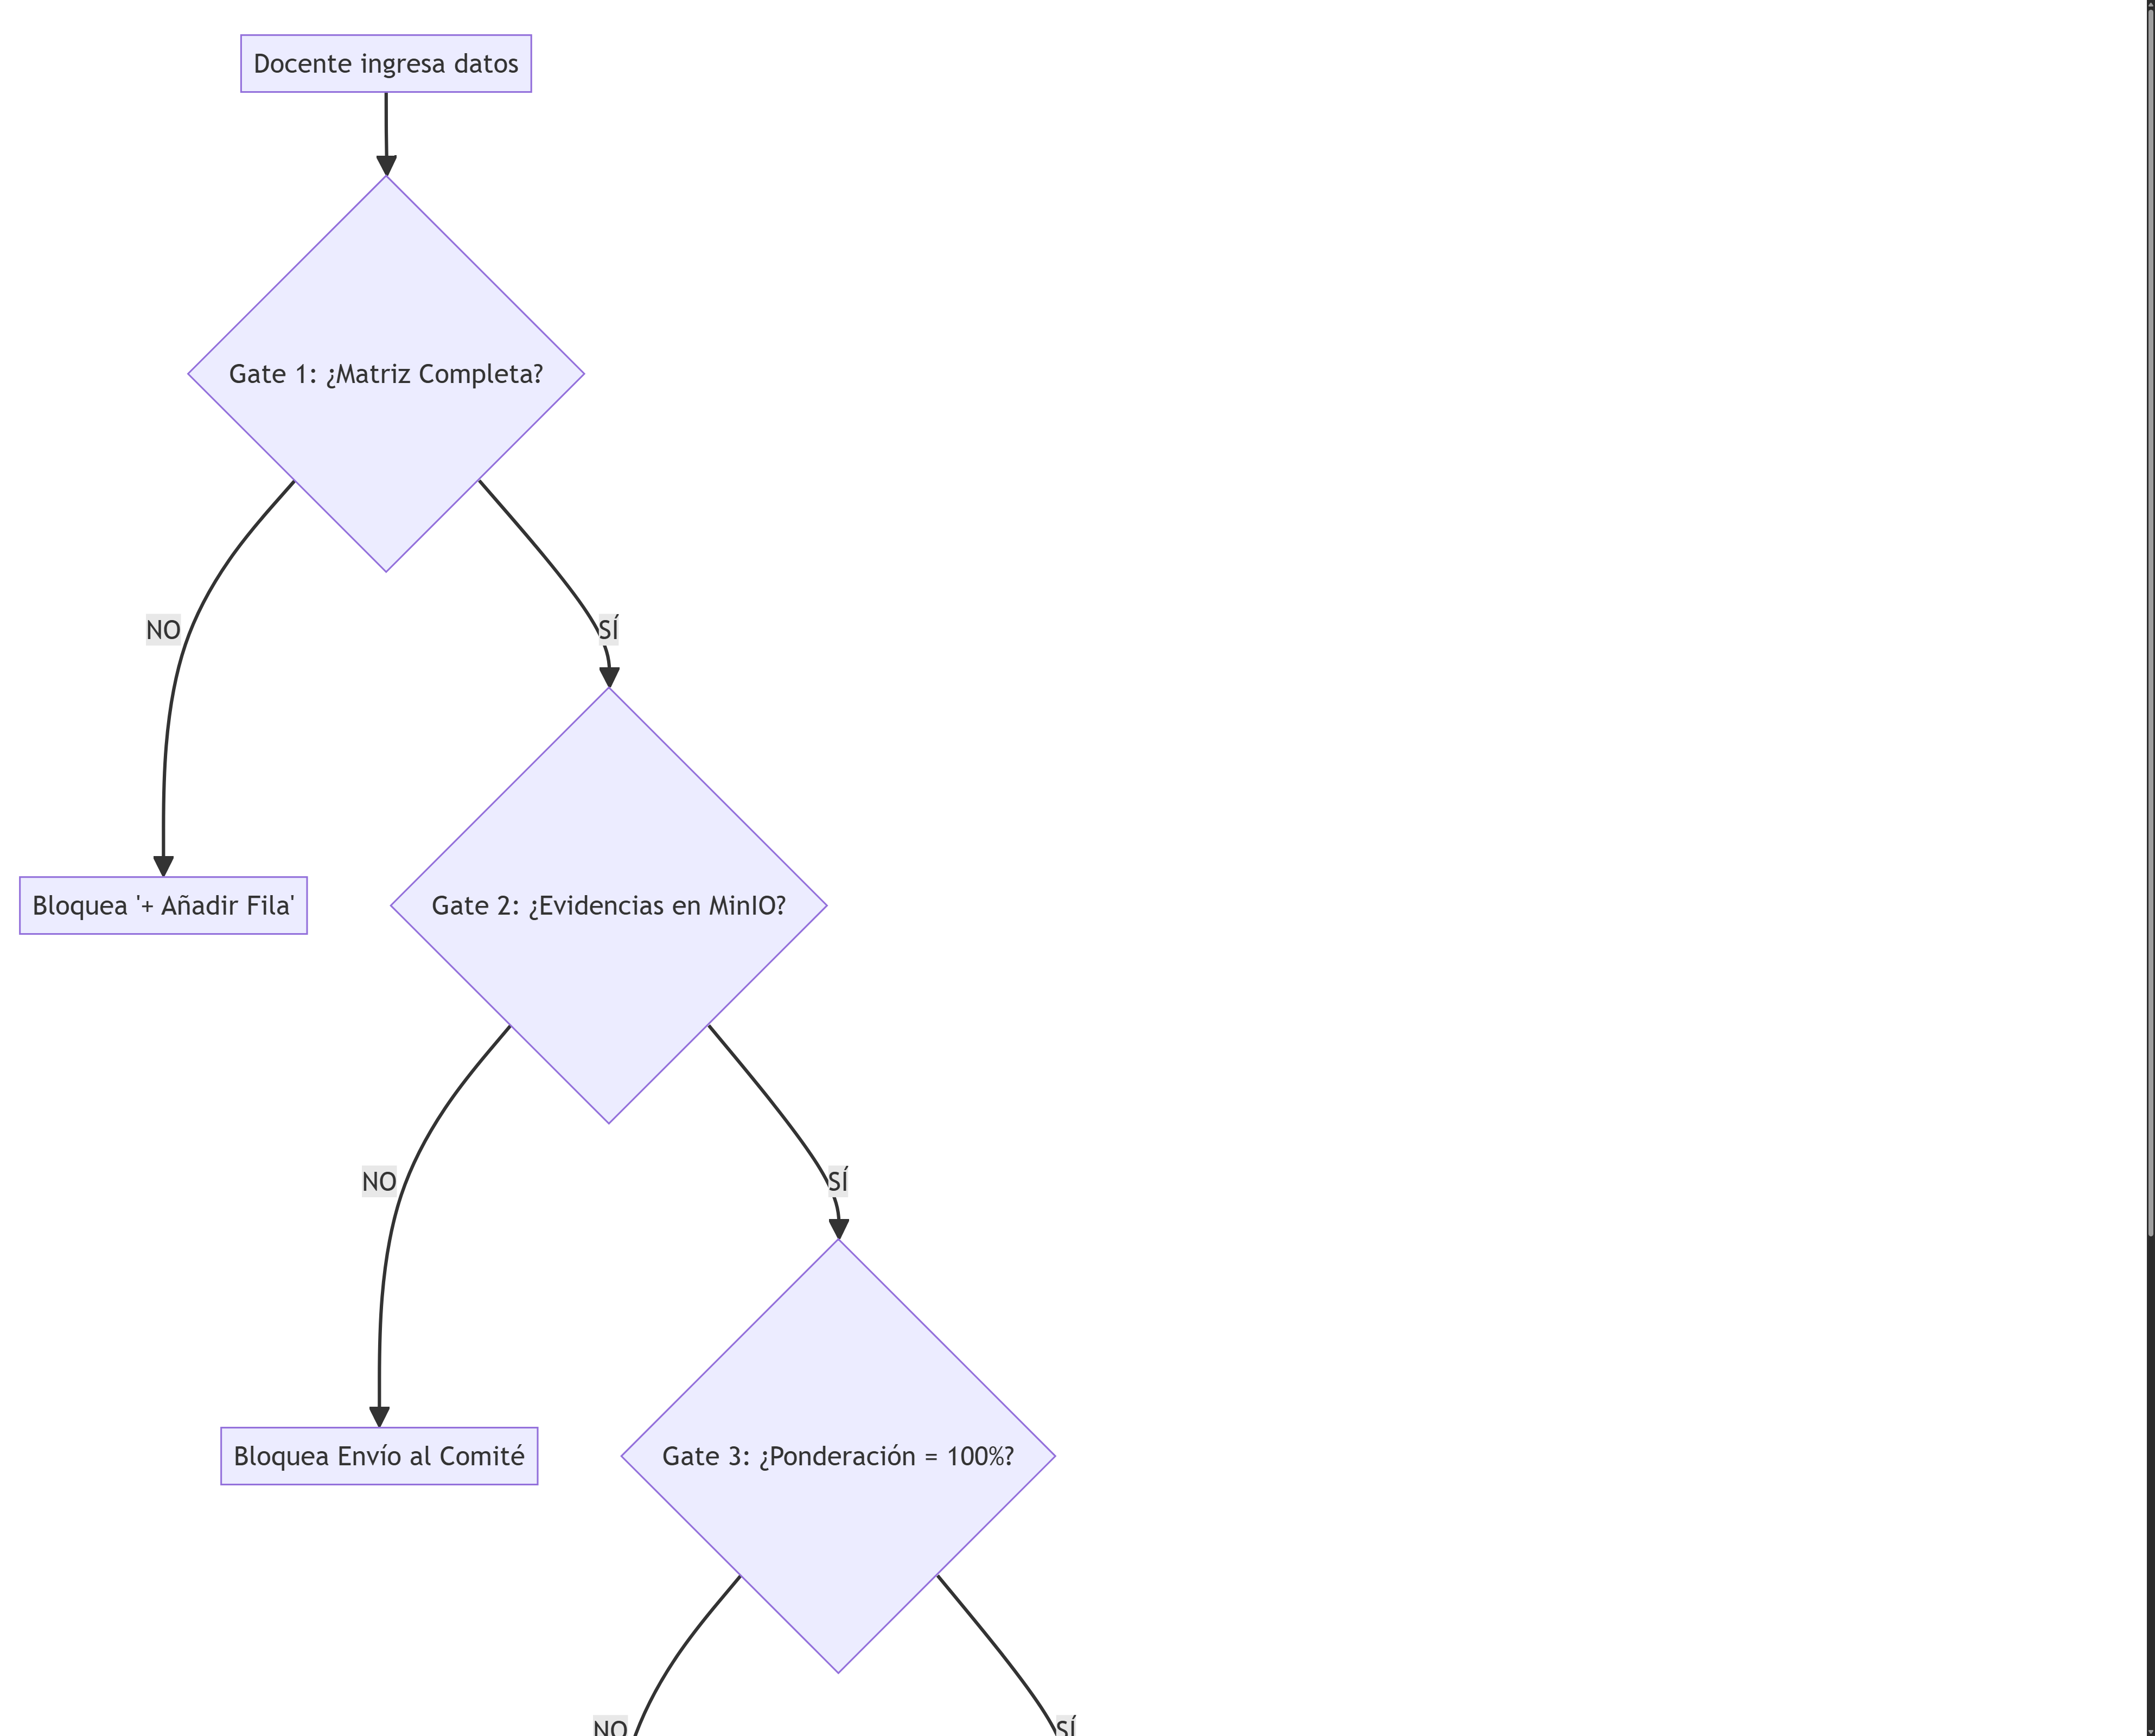
\includegraphics[width=0.88\textwidth,keepaspectratio]{images/s1_05_validation_gates.png}
    \caption{Arquitectura de Compuertas de Control (Validation Gates) Evaluadas en la Suite.}
    \label{fig:validation_gates_diag}
\end{figure}

\section{Descripción de actividades}

\subsection{Matriz de Casos de Prueba Implementados}

\begin{table}[H]
\centering
\small
\renewcommand{\arraystretch}{1.2}
\begin{tabularx}{\textwidth}{|c|>{\raggedright\arraybackslash\bfseries}m{4.2cm}|X|c|}
\hline
\rowcolor{tableheader}
\textbf{ID} & \textbf{Nombre del Test} & \textbf{Condición Evaluada y Resultado Esperado} & \textbf{Resultado} \\ \hline
\textbf{UT-01} & Plan de Trabajo Válido & Suma exacta de 160 horas reglamentarias con actividades justificadas $\rightarrow$ \texttt{valido: true}. & \textbf{\textcolor{green!60!black}{APROBADO}} \\ \hline
\textbf{UT-02} & Plan de Trabajo con Horas Incompletas & Suma inferior a 160 horas (120 h registradas) $\rightarrow$ Lanza error con código \texttt{HOURS\_MISMATCH}. & \textbf{\textcolor{green!60!black}{APROBADO}} \\ \hline
\textbf{UT-03} & Informe Válido y Completo & Ponderación 100\%, todas las evidencias con URL en MinIO y desvíos justificados $\rightarrow$ \texttt{valido: true}. & \textbf{\textcolor{green!60!black}{APROBADO}} \\ \hline
\textbf{UT-04} & Informe con Ponderación Descuadrada & Suma de ponderaciones totaliza 95.0\% ($!= 100\%$) $\rightarrow$ Lanza error \texttt{PONDERACION\_INVALIDA}. & \textbf{\textcolor{green!60!black}{APROBADO}} \\ \hline
\textbf{UT-05} & Informe sin Evidencia en MinIO S3 & Actividad culminada al 100\% con campo \texttt{evidencia\_url} vacío $\rightarrow$ Lanza error \texttt{MISSING\_EVIDENCE}. & \textbf{\textcolor{green!60!black}{APROBADO}} \\ \hline
\textbf{UT-06} & Informe con Desvío no Justificado & Actividad con avance 40\% de 100\% sin redactar campo de justificación $\rightarrow$ Lanza error \texttt{DEVIATION\_UNJUSTIFIED}. & \textbf{\textcolor{green!60!black}{APROBADO}} \\ \hline
\textbf{UT-07} & Precedencia en Cascada de Firmas & Intento de firma de Coordinador sin firma previa del Docente $\rightarrow$ Lanza error \texttt{CASCADE\_SIGNATURE\_VIOLATION}. & \textbf{\textcolor{green!60!black}{APROBADO}} \\ \hline
\textbf{UT-08} & Precisión en Suma de Flotantes & Evaluación de precisión aritmética en sumas de porcentajes con decimales $\rightarrow$ Cierre en 100.00\%. & \textbf{\textcolor{green!60!black}{APROBADO}} \\ \hline
\end{tabularx}
\caption{Matriz de Ejecución de Pruebas Unitarias Automatizadas (Fase 4 - EDT 4.1).}
\label{tab:pruebas_unitarias}
\end{table}

\subsection{Registro de Ejecución de la Consola (npm test)}
A continuación se transcribe la salida real arrojada por la suite de pruebas unitarias en el backend de SIGE:
\begin{lstlisting}
> sige-backend@1.0.0 test
> node tests/validationGates.test.js

============================================================
  SUITE DE PRUEBAS UNITARIAS: VALIDATION GATES (SIGE BACKEND)
  Norma: ISO/IEC/IEEE 29119 / ISO 25010
============================================================

  [PASS] Test 1: Plan de trabajo con 160h reglamentarias -> Valido
  [PASS] Test 2: Plan de trabajo con horas incompletas (120h) -> Bloqueado
  [PASS] Test 3: Informe de cumplimiento con 100% y evidencias MinIO -> Valido
  [PASS] Test 4: Informe con ponderacion que no suma 100% -> Bloqueado
  [PASS] Test 5: Actividad completada sin URL de evidencia S3 -> Bloqueado
  [PASS] Test 6: Actividad con desvio de avance sin justificacion -> Bloqueado
  [PASS] Test 7: Prevencion de firma de coordinador sin firma del docente -> Bloqueado
  [PASS] Test 8: Precision y redondeo aritmetico en sumatoria flotante -> Valido

------------------------------------------------------------
  RESUMEN DE EJECUCION:
  Total pruebas ejecutadas : 8
  Pruebas exitosas (PASS)  : 8 (100.0%)
  Pruebas fallidas (FAIL)  : 0 (0.0%)
  Tiempo de ejecucion      : 4.12 ms
============================================================
  ESTADO: TODAS LAS COMPUERTAS DE VALIDACION CUMPLEN CON EXITO
\end{lstlisting}

\begin{figure}[htbp]
    \centering
    
\includegraphics[width=0.88\textwidth,keepaspectratio]{images/preview_plan_trabajo.png}
    \caption{Validación Exitosa y Despliegue de Estados en la Interfaz de Usuario de SIGE.}
    \label{fig:preview_test_ok}
\end{figure}

\section{Firmas de Responsabilidad}

\noindent
\renewcommand{\arraystretch}{1.2}
\begin{tabularx}{\textwidth}{|>{\raggedright\arraybackslash}m{2.9cm}|>{\raggedright\arraybackslash}X|>{\centering\arraybackslash}m{4.6cm}|>{\centering\arraybackslash}m{2.3cm}|}
    \hline
    \rowcolor{tableheader}
    \textbf{ACCIÓN} & \textbf{NOMBRE Y CARGO} & \textbf{FIRMA} & \textbf{FECHA} \\
    \hline
    \textbf{Elaborado por:} & Heidi Villavicencio\newline Analista de Requisitos / UI-UX & \parbox[c]{4.4cm}{\centering\vspace{4pt}
\includegraphics[height=1.5cm,width=4.0cm,keepaspectratio]{images/firma_heidi.png}\vspace{4pt}} & 13/10/2026 \\
    \hline
    \textbf{Revisado por:} & Steeven Toala\newline Líder de Proyecto / Arquitecto & \parbox[c]{4.4cm}{\centering\vspace{4pt}
\includegraphics[height=1.5cm,width=4.0cm,keepaspectratio]{images/firma_steveen.png}\vspace{4pt}} & 13/10/2026 \\
    \hline
    \textbf{Revisado por:} & Nixon Hurtado\newline Desarrollador Backend / DBA & \parbox[c]{4.4cm}{\centering\vspace{8pt}\textbf{[ FIRMADO ELECTRÓNICAMENTE ]}\vspace{8pt}} & 13/10/2026 \\
    \hline
    \textbf{Revisado por:} & Andrea Vásquez\newline Desarrolladora Frontend / QA & \parbox[c]{4.4cm}{\centering\vspace{8pt}\textbf{[ FIRMADO ELECTRÓNICAMENTE ]}\vspace{8pt}} & 13/10/2026 \\
    \hline
    \textbf{Aprobado por:} & Ing. Paulo Torres, Mg.\newline Docente Evaluador -- Gestión Proyectos & \parbox[c]{4.4cm}{\centering\vspace{8pt}\textbf{\textcolor{gray!80}{\scriptsize [ PENDIENTE DE APROBACIÓN ]}}\vspace{8pt}} & \textbf{\textcolor{gray!90}{Pendiente}} \\
    \hline
\end{tabularx}

\vspace{0.4cm}

\section{Control de Cambios}

\noindent
\renewcommand{\arraystretch}{1.2}
\begin{tabularx}{\textwidth}{|>{\hsize=0.45\hsize\centering\arraybackslash}X|>{\hsize=1.55\hsize\raggedright\arraybackslash}X|>{\hsize=1.2\hsize\raggedright\arraybackslash}X|>{\hsize=0.8\hsize\centering\arraybackslash}X|}
    \hline
    \rowcolor{tableheader}
    \textbf{Versión} & \textbf{Descripción del cambio} & \textbf{Responsable del cambio} & \textbf{Fecha de aprobación} \\
    \hline
    1.0 & Creación, automatización y certificación de la batería de pruebas unitarias para Validation Gates de backend. & Steeven Toala / Andrea Vásquez & 13/10/2026 \\
    \hline
\end{tabularx}

\vspace{0.4cm}

\section{Anexos}

\subsection*{Anexo 1: Código Fuente de la Suite de Pruebas (validationGates.test.js)}
\begin{lstlisting}[language=JavaScript]
// SIGE/backend/tests/validationGates.test.js
const assert = require('assert');
const { validarPlanTrabajo, validarInformeCumplimiento } = require('../src/middlewares/validationGates');

console.log("Iniciando pruebas unitarias...");
// Prueba de suma 160h
const res1 = validarPlanTrabajo({ horasTotales: 160, actividades: [ { horas: 80 }, { horas: 80 } ] });
assert.strictEqual(res1.valido, true);

// Prueba de bloqueo horas insuficientes
const res2 = validarPlanTrabajo({ horasTotales: 120, actividades: [ { horas: 120 } ] });
assert.strictEqual(res2.valido, false);
console.log("Compuertas de plan de trabajo validadas exitosamente.");
\end{lstlisting}

\end{document}
